\documentclass[tikz,border=5mm]{standalone}
\usepackage{tikz}
\usepackage{amsmath}
\usetikzlibrary{positioning, arrows.meta, calc, decorations.pathreplacing}

%% Fonts
\usepackage{helvet}
\renewcommand{\familydefault}{\sfdefault}
\usepackage{sansmath}
\sansmath

%% Colors
\definecolor{colour_calc}{HTML}{35b779}
\definecolor{colour_exp}{HTML}{ff991c}
\definecolor{colour_ie}{HTML}{31688e}

\begin{document}
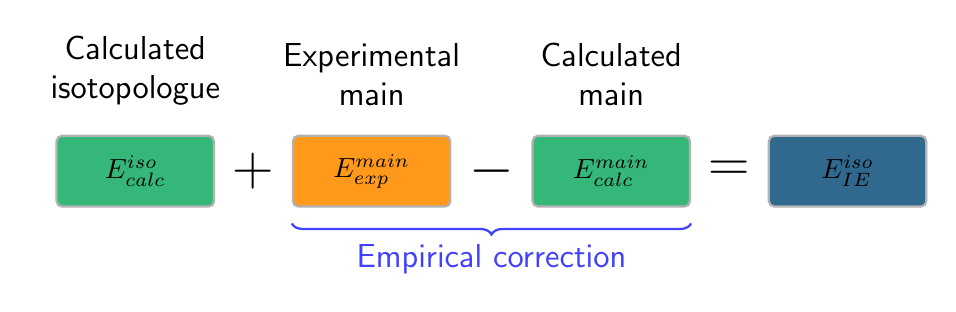
\begin{tikzpicture}[
    font=\sffamily,
    box/.style={rectangle, draw=gray!60, thick, rounded corners=2pt,
                minimum height=0.9cm, minimum width=2cm, align=center},
    arrow/.style={-{Latex[length=2mm]}, thick, gray!70},
    calc/.style={fill=colour_calc},
    exp/.style={fill=colour_exp},
    ie/.style={fill=colour_ie}
]

% Main equation boxes
\node[box, calc] (iso) {$E_{calc}^{iso}$};
\node[font=\huge, right=0.1cm of iso] (plus) {$+$};
\node[box, exp, right=0.1cm of plus] (exp) {$E_{exp}^{main}$};
\node[font=\huge, right=0.1cm of exp] (minus) {$-$};
\node[box, calc, right=0.1cm of minus] (calc) {$E_{calc}^{main}$};
\node[font=\huge, right=0.1cm of calc] (equals) {$=$};
\node[box, ie, right=0.1cm of equals] (result) {$E_{IE}^{iso}$};

% Labels above
\node[above=0.25cm of iso, font=\large, text width=2.5cm, align=center] 
     {Calculated\\isotopologue};
\node[above=0.25cm of exp, font=\large, text width=2.5cm, align=center] 
     {Experimental\\main};
\node[above=0.25cm of calc, font=\large, text width=2.5cm, align=center] 
     {Calculated\\main};

% Brace showing correction
\draw[decorate, decoration={brace, amplitude=4pt, mirror}, thick, blue!75]
($(exp.south west)+(0,-0.2)$) -- ($(calc.south east)+(0,-0.2)$)
node[midway, below=4pt, font=\large, text=blue!75]
{Empirical correction};

\end{tikzpicture}
\end{document}